\chapter{Closures and Iterators}

\section{Introduction to Closures}

In system programming, there are many scenarios where we need to pass behavior as an argument to another function. Think of a sorting algorithm where you need to specify a custom comparison rule, or a thread that needs to execute a specific task. While traditional functions can be passed around via function pointers, they have a critical limitation: they cannot easily capture variables from the environment where they are defined.

This is the problem that \textbf{closures} solve. A closure is an anonymous function that can capture variables from its surrounding lexical scope. You can think of a closure as a regular function equipped with a "backpack" containing the data it captured from its environment.

\subsection{Building Intuition: Capturing the Environment}

When you define a closure in Rust, the compiler automatically creates an anonymous \texttt{struct} under the hood. This struct contains the variables that the closure captures. Depending on how the closure uses these variables, they are captured either by shared reference, mutable reference, or by value (ownership transfer).

\begin{lstlisting}[language=Rust]
let y = 10;
let z = 20;

// A closure capturing y and z by reference
let add_refs = |x| {
    x + y + z 
};

println!("Result: {}", add_refs(5)); // Output: 35
\end{lstlisting}

\textbf{Deep Memory Model Analysis:} When the closure \texttt{add\_refs} is created, the compiler allocates an anonymous struct on the stack. Because \texttt{y} and \texttt{z} are only read, this struct contains two immutable references: \texttt{\&i32} pointing to \texttt{y} and \texttt{\&i32} pointing to \texttt{z}. No heap allocation occurs here. The closure's lifetime is implicitly bounded by the lifetimes of \texttt{y} and \texttt{z}. When \texttt{add\_refs} is invoked, it accesses these stack-allocated integers via the stored references without taking ownership.

\begin{notebox}
The compiler infers how variables should be captured by looking at what the closure does with them. If you only read \texttt{y} and \texttt{z}, they are captured as immutable references (\texttt{\&y}, \texttt{\&z}).
\end{notebox}

If the closure modifies a captured variable, it implicitly captures a mutable reference.

\begin{lstlisting}[language=Rust]
let mut sum = 0;
// Captures `sum` by mutable reference
let mut accumulate = |x| {
    sum += x;
};

accumulate(5);
accumulate(7);
println!("Sum: {}", sum); // Output: 12
\end{lstlisting}

\begin{insightbox}
\textbf{Mental Model: Closures as Structs} \\
When you write \texttt{|x| \{ sum += x \}}, Rust generates a struct holding \texttt{\&mut i32} (pointing to \texttt{sum}). The closure itself is just an instance of this struct that implements a specific trait to become callable.
\end{insightbox}

Sometimes, especially when returning a closure from a function or sending it to another thread, you want the closure to take full ownership of the captured variables. You force this behavior using the \texttt{move} keyword.

\begin{notebox}
\textbf{Lifetimes and \texttt{move}:} Without \texttt{move}, a closure captures variables by reference, meaning the closure's lifetime is strictly tied to (and cannot outlive) the shortest-lived captured reference. Using \texttt{move} makes the closure self-sufficient. Also, note that using \texttt{move} forces capture by value, but it \textit{does not} automatically make the closure \texttt{FnOnce}. The trait implemented still depends entirely on how the captured value is used inside the closure's body.
\end{notebox}

\begin{lstlisting}[language=Rust]
let prefix = String::from("ID_");

// `move` forces the closure to take ownership of `prefix`
let generate_id = move |i| {
    format!("{}{}", prefix, i)
};

// prefix is no longer accessible here!
\end{lstlisting}

\textbf{Deep Memory Model Analysis:} Here, the \texttt{String} \texttt{prefix} is a fat pointer on the stack (containing a pointer, length, and capacity) that manages a heap-allocated UTF-8 buffer. By using \texttt{move}, the ownership of the \texttt{String} is transferred entirely into the closure's anonymous struct. The struct is created on the stack containing the \texttt{String} fat pointer. As a result, the original \texttt{prefix} variable becomes uninitialized (moved). When the closure is eventually dropped, it will drop the \texttt{String}, deallocating the heap buffer. The closure now dictates the lifetime of the data, making it "self-sufficient" and safe to return or pass to other threads.

\subsection{The Closure Traits: \texttt{FnOnce}, \texttt{FnMut}, and \texttt{Fn}}

Rust formalizes the behavior of closures through three functional traits. These traits dictate what the closure is allowed to do with its captured environment and how many times it can be called.

\begin{itemize}
    \item \texttt{FnOnce}: The most general closure type. It consumes its captured variables. Because it consumes them, it can be called \textbf{strictly once}. All closures implement \texttt{FnOnce}.
    \item \texttt{FnMut}: A closure that can mutate its captured variables. It can be called multiple times. It requires \texttt{\&mut self} to be executed.
    \item \texttt{Fn}: A closure that only reads its captured variables (or captures nothing at all). It can be called multiple times without modifying its state. It takes \texttt{\&self}.
\end{itemize}

\begin{exambox}
\textbf{Exam Tip}: Remember the hierarchy of closure traits: \texttt{Fn} is a sub-trait of \texttt{FnMut}, which is a sub-trait of \texttt{FnOnce}. A function that expects an \texttt{FnOnce} can accept any closure, but a function expecting an \texttt{Fn} is the most restrictive.
\end{exambox}

\subsection{Passing and Returning Closures}

When a function accepts a closure, it can do so using \textbf{Generics} (static dispatch) or \textbf{Trait Objects} (dynamic dispatch).

\begin{examprioritybox}
\textbf{Common Pitfall:} Confusing when to use generics vs. trait objects for closures, resulting in either code bloat or unnecessary runtime overhead.
\textbf{Expected Mastery Level:} High. You must be able to justify your choice between monomorphization and dynamic dispatch.

\textbf{Using Generics (Static Dispatch):}
\begin{lstlisting}[language=Rust]
// We don't care about the specific type F, as long as it implements Fn
fn apply<F>(value: i32, f: F) -> i32 
where 
    F: Fn(i32) -> i32 
{
    f(value)
}

let squared = apply(5, |x| x * x); // Generates apply_square
let halved  = apply(10, |x| x / 2); // Generates apply_divide
let inc     = apply(3, |x| x + 1); // Generates apply_increment
\end{lstlisting}
\textit{Trade-off}: Generics generate specialized machine code for every unique closure passed to \texttt{apply} (a process called monomorphization). For instance, the compiler will generate three completely distinct copies of the \texttt{apply} function under the hood (e.g., \texttt{apply\_square}, \texttt{apply\_divide}, \texttt{apply\_increment}). This makes it extremely fast (often inlined), but can slightly increase compile times and binary size.

\textbf{Using Trait Objects (Dynamic Dispatch):}
\begin{lstlisting}[language=Rust]
struct PipelineStep {
    // We use a Boxed trait object to store ANY closure of this signature
    op: Box<dyn Fn(i32) -> i32>,
}
\end{lstlisting}
\textit{Trade-off}: Trait objects encapsulate the closure behind a pointer (a fat pointer containing the closure data and a vtable). \textbf{Deep Memory Model Analysis:} The vtable for a closure in this context typically contains exactly four entries: a pointer to the \texttt{drop} logic, the \texttt{size} of the captured data, its \texttt{align}ment, and the pointer to the actual anonymous method to execute. This is slightly slower due to pointer indirection (cache misses as the CPU jumps to the vtable and then the code---as the professor noted, "skipping two steps breaks the location of the cache a bit, we're talking about nanoseconds"). However, its major advantage is \textbf{homogeneity}. It allows storing heterogeneous closures (e.g., an addition closure, a multiplication closure) in a single collection like \texttt{Vec<Box<dyn Fn(...)>>} to build flexible execution pipelines.
\end{examprioritybox}

\begin{examprioritybox}
\textbf{Common Pitfall:} Forgetting the \texttt{move} keyword when returning a closure, leading to "borrowed value does not live long enough" compiler errors.
\textbf{Expected Mastery Level:} Very High. Returning stateful closures (generators) is a heavily emphasized exam pattern.

\textbf{Returning Closures (Generators):}
When a function returns a closure, the exact type of the closure is unknown at compile time. Thus, we must use the \texttt{impl Trait} syntax (e.g., \texttt{impl Fn() -> T}).

\begin{lstlisting}[language=Rust]
// Returns a closure that yields copies of the captured value `v`
fn value_source<T: Clone>(v: T) -> impl Fn() -> T {
    // `move` is essential here to take ownership of `v`
    move || v.clone() 
}
\end{lstlisting}

\begin{warningbox}
\textbf{The "Dangling" Threat:} If we did not use \texttt{move}, the closure would try to capture \texttt{v} by reference. However, \texttt{v} is a parameter local to the function's stack frame. As soon as the function returns, that stack frame is destroyed. Any returned reference would become \textit{dangling}, pointing to invalid memory. The \texttt{move} keyword forces the closure to take full possession of the value ("diventa mio, me lo copio"), making it self-sufficient.
\end{warningbox}

Returning a closure is also a common pattern for creating stateful generators. This approach neatly encapsulates internal state without requiring you to define an explicit \texttt{struct}.

\begin{lstlisting}[language=Rust]
fn create_generator(prefix: String) -> impl FnMut() -> String {
    let mut i = 0;
    // `move` ensures `prefix` and `i` are moved into the closure
    move || {
        i += 1;
        format!("{}{}", prefix, i)
    }
}

let mut gen = create_generator(String::from("User_"));
println!("{}", gen()); // User_1
println!("{}", gen()); // User_2
\end{lstlisting}

\textbf{Deep Memory Model Analysis:} When \texttt{create\_generator} is called, \texttt{prefix} (a \texttt{String} with a heap allocation) and \texttt{i} (an \texttt{i32}) are created on the stack frame of the function. The \texttt{move} keyword forces the closure to take ownership. A new anonymous struct implementing \texttt{FnMut} is created, and the \texttt{String} fat pointer and the integer are moved into this struct. The function then returns this struct (its size is statically known to the compiler, so it is returned on the stack). Each time the closure is called, it mutates its internal \texttt{i} state directly in its struct memory and allocates a new \texttt{String} on the heap to return.
\end{examprioritybox}

\section{Iterators: The Core Concept}

Most algorithms involve looping over data. The traditional \texttt{for} or \texttt{while} loops with index increments work well for simple arrays, but they expose the internal structure of the collection. What if we want to iterate over a tree, a linked list, or a hash map? 

The \textbf{Iterator} pattern solves this. An iterator is an object that provides a uniform interface to traverse a sequence of elements, regardless of how those elements are stored or generated. This explicit representation of operations over a sequence also lends itself exceptionally well to performance optimizations. For example, using dedicated libraries like \texttt{rayon}, it is trivial to transform a sequential iterator pipeline into a parallel one that exploits multi-core processors.

\subsection{The \texttt{Iterator} Trait}

In Rust, the Iterator mechanism is shockingly simple. While many other languages separate the check for more elements (\texttt{hasNext()}) and the retrieval (\texttt{next()}), Rust combines both into a single \texttt{next} method.

\begin{lstlisting}[language=Rust]
pub trait Iterator {
    type Item; // The type of element being iterated
    
    // Returns `Some(Item)` if there is an element, or `None` if finished
    fn next(&mut self) -> Option<Self::Item>;
}
\end{lstlisting}

When \texttt{next()} returns \texttt{Some(value)}, you have a value. When it returns \texttt{None}, the iterator is exhausted. Calling \texttt{next()} again after \texttt{None} will typically just return \texttt{None} forever.

\subsection{Iteration Modes}

Collections typically provide three ways to create an iterator, corresponding to the three modes of ownership:

1. \texttt{iter()}: Returns an iterator over shared references (\texttt{\&T}). The original collection remains intact and immutable.
2. \texttt{iter\_mut()}: Returns an iterator over mutable references (\texttt{\&mut T}). Useful for modifying elements in place.
3. \texttt{into\_iter()}: Returns an iterator that takes ownership of the collection, yielding owned values (\texttt{T}). The original collection is consumed and destroyed.

\begin{notebox}
Note that not all collections support all three modes identically. For instance, \texttt{HashMap} and \texttt{BTreeMap} do not provide a way to iterate \textit{mutably} over their keys. Mutating a key in-place would break the underlying data structure's invariants.
\end{notebox}

\begin{examprioritybox}
\textbf{Common Pitfall:} Using a \texttt{for} loop directly on a collection (\texttt{for x in v}) when you meant to only read it (\texttt{for x in \&v}), accidentally consuming and destroying the container.
\textbf{Expected Mastery Level:} High. You must instinctively know whether an iteration yields \texttt{T}, \texttt{\&T}, or \texttt{\&mut T}.

\begin{lstlisting}[language=Rust]
let mut v = vec![String::from("A"), String::from("B")];

// 1. Immutable Iteration
for s in v.iter() {
    println!("{}", s); // s is &String
}

// 2. Mutable Iteration
for s in v.iter_mut() {
    s.push_str("1"); // s is &mut String
}

// 3. Consuming Iteration
for s in v.into_iter() {
    println!("{}", s); // s is String (moved)
}
// `v` is no longer valid here!
\end{lstlisting}

\textbf{Deep Memory Model Analysis:} 
\begin{itemize}
    \item \texttt{v.iter()}: Creates an iterator struct on the stack containing a pointer to the vector's heap buffer and an index. It yields \texttt{\&String} references. No heap data is duplicated or dropped.
    \item \texttt{v.iter\_mut()}: Similar to \texttt{iter()}, but yields \texttt{\&mut String} references. It relies on unsafe code under the hood to split the mutable borrow safely, ensuring no two mutable references point to the same element.
    \item \texttt{v.into\_iter()}: The vector is "disassembled". The iterator takes ownership of the vector's heap buffer. As it iterates, it yields the actual \texttt{String} structs (fat pointers) to the caller. Once iteration finishes, the iterator drops the remaining un-yielded elements and deallocates the vector's heap buffer itself.
\end{itemize}
\end{examprioritybox}

\begin{notebox}
\textbf{The \texttt{for} Loop Sugar}: Under the hood, Rust's \texttt{for} loop is syntactic sugar. It calls \texttt{IntoIterator::into\_iter()} on the collection to get an iterator, and then repeatedly calls \texttt{next()} until it hits \texttt{None}. 
\end{notebox}

\section{The Iterator Pipeline: Adapters and Consumers}

The true power of iterators in Rust comes from combinability. The \texttt{Iterator} trait has over 50 default methods (adapters and consumers) that allow you to chain operations elegantly.

\subsection{Lazy Evaluation}

Iterators in Rust are \textbf{lazy}. This means that creating an iterator and chaining adapters does absolutely nothing until a \textit{consumer} is called.

\begin{figure}[h]
    \centering
    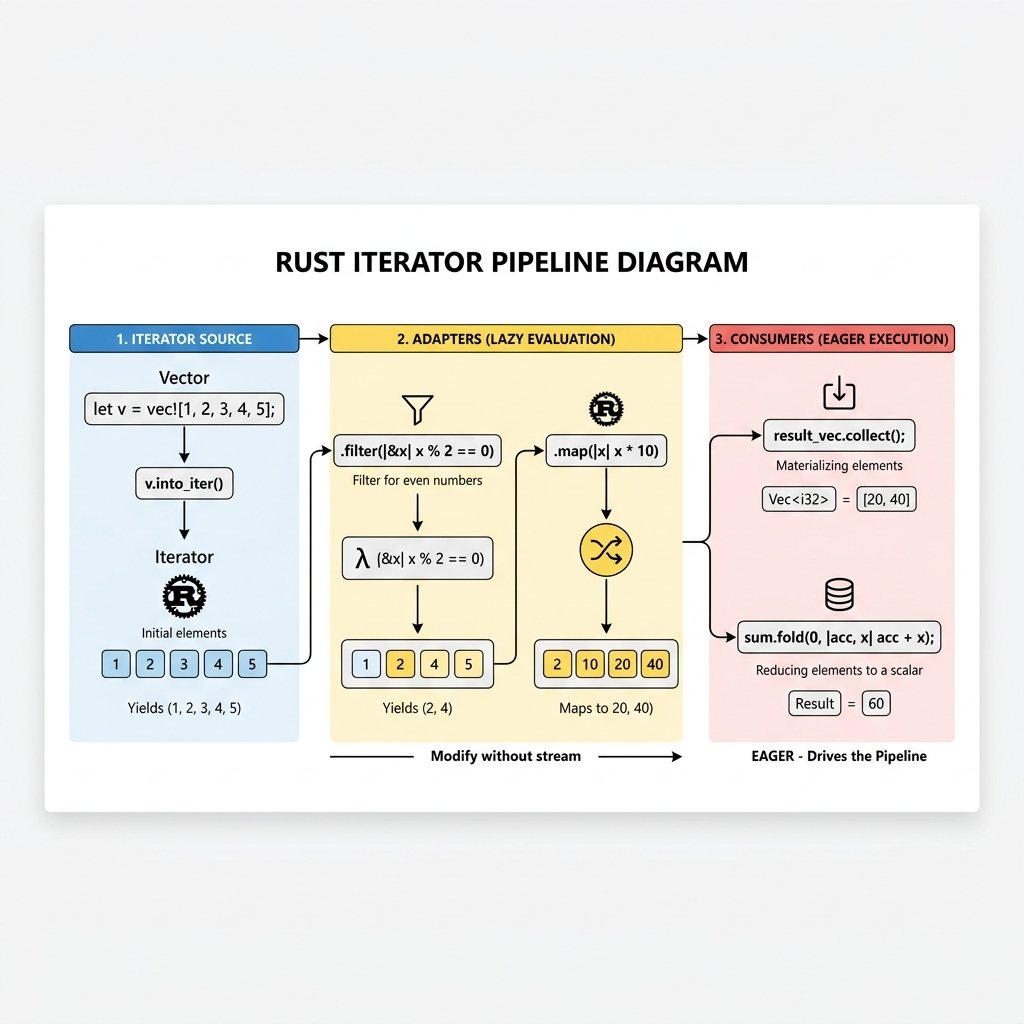
\includegraphics[width=0.8\textwidth]{images/iterator_pipeline.png}
    \caption{The Iterator Pipeline: Adapters chain lazily, and Consumers drive the execution.}
    \label{fig:iterators}
\end{figure}

\begin{insightbox}
\textbf{Professor's Analogy: Ordering a Custom Car} \\
Iterators are entirely lazy. They simply prepare the pipeline but perform no work until requested. It's like buying a custom car: you place the order and the manufacturer says, "It will arrive in six months." Why? Because car manufacturers learned it's not cost-effective to pre-build everything and risk it sitting unsold. It's much better to wait for someone to actually request it, provide the money, and \textit{only then} start the production process. Similarly, iterators avoid spending CPU cycles on elements you might never actually use!
\end{insightbox}

\begin{examprioritybox}
\textbf{Common Pitfall:} Creating complex iterator adapters but forgetting to call a consumer, meaning the iteration code never actually executes.
\textbf{Expected Mastery Level:} High. Understand how the request for an element propagates strictly from the consumer back up to the source.

Think of an iterator pipeline as a plumbing system. You can connect hoses and valves (adapters like \texttt{map} and \texttt{filter}) all you want, but no water will flow. It's only when you open the tap at the very end of the line (a consumer like \texttt{collect}) that the system activates. The consumer asks the last adapter for an element, which in turn asks the previous one, propagating the request all the way up to the source container. Elements are processed strictly on-demand. This zero-cost abstraction ensures that we don't perform unnecessary work or allocate intermediate collections in memory.
\end{examprioritybox}

\subsection{Adapters}

Adapters are methods that take an iterator and return a \textit{new} iterator.
\begin{itemize}
    \item \texttt{map(|x| ...)}: Applies a closure to every element, transforming it.
    \item \texttt{filter(|x| ...)}: Keeps only elements for which the closure returns \texttt{true}.
    \item \texttt{enumerate()}: Yields \texttt{(index, value)} pairs.
    \item \texttt{take(n)}: Yields the first $n$ elements, then stops.
    \item \texttt{take\_while(|x| ...)}: Continues yielding elements as long as the condition returns \texttt{true}, then stops.
    \item \texttt{skip(n)}: Ignores the first $n$ elements, then yields the rest.
    \item \texttt{skip\_while(|x| ...)}: Ignores elements as long as the condition is \texttt{true}, then yields all remaining elements.
    \item \texttt{chain(other)}: Appends another iterator to the end of this one.
    \item \texttt{zip(other)}: Pairs up elements from two iterators into tuples.
    \item \texttt{rev()}: Reverses the direction of iteration (requires the underlying iterator to support moving backwards).
    \item \texttt{flatten()}: Removes one level of nesting (e.g., turns an iterator of lists into an iterator of elements).
    \item \texttt{flat\_map(|x| ...)}: Applies a function that returns an iterator, and then flattens the result.
    \item \texttt{filter\_map(|x| ...)}: A concise combination of \texttt{filter} and \texttt{map} that yields elements for which the closure returns \texttt{Some}.
    \item \texttt{inspect(|x| ...)}: Allows you to examine the element (e.g., for \texttt{println!} debugging) without modifying or consuming it.
    \item \texttt{fuse()}: Creates an iterator that will definitively yield \texttt{None} forever after yielding \texttt{None} once, ensuring predictable termination.
    \item \texttt{cloned() / copied()}: Creates an iterator that clones or copies the elements, turning an iterator of references into owned values.
\end{itemize}

\subsection{Consumers}

Consumers are methods that call \texttt{next()} on the iterator pipeline and produce a final value.
\begin{itemize}
    \item \texttt{collect()}: Gathers all elements into a collection (e.g., a \texttt{Vec} or \texttt{HashMap}).
    \item \texttt{sum()}, \texttt{product()}, \texttt{count()}, \texttt{min()}, \texttt{max()}: Perform common aggregations.
    \item \texttt{fold(init, |acc, x| ...)}: The mother of all consumers, applying an accumulator.
    \item \texttt{try\_fold(init, |acc, x| ...)}: A variant of \texttt{fold} that halts immediately if an error (\texttt{Err} or \texttt{None}) is encountered.
    \item \texttt{reduce(|acc, x| ...)}: Similar to \texttt{fold}, but uses the first element of the sequence as the initial value, returning an \texttt{Option}.
    \item \texttt{partition(|x| ...)}: Splits the elements into a tuple of two collections: those that satisfy the predicate and those that don't.
\end{itemize}

\begin{lstlisting}[language=Rust]
let numbers = vec![1, 2, 3, 4, 5, 6];

// The adapters do nothing until collect() is called
let even_squares: Vec<i32> = numbers.into_iter()
    .filter(|&x| x % 2 == 0) // keeps 2, 4, 6
    .map(|x| x * x)          // turns to 4, 16, 36
    .collect();              // drives the pipeline
\end{lstlisting}

\begin{warningbox}
Because iterators are lazy, if you write a map operation that produces side effects (like printing to the console) but you never call a consumer at the end, the code will compile but \textit{nothing will happen}. The compiler will issue a "must use" warning.
\end{warningbox}

\subsection{Understanding \texttt{fold}}

\begin{examprioritybox}
\textbf{Common Pitfall:} Trying to use mutable external variables to accumulate a sum or product in an iterator pipeline instead of using \texttt{fold}.
\textbf{Expected Mastery Level:} Very High. The professor explicitly calls this "the basis of computation" and the most powerful method of all iterators. 

The \texttt{fold} method is the fundamental aggregation operation. It's conceptually similar to the accumulator register in a CPU. It starts with an initial value, and applies a function to combine the accumulator with every element from the iterator. All other consumers could theoretically be implemented using \texttt{fold}.

\begin{lstlisting}[language=Rust]
let v = vec![1, 2, 3];
// sum starts at 0. 
// step 1: acc(0) + x(1) -> 1
// step 2: acc(1) + x(2) -> 3
// step 3: acc(3) + x(3) -> 6
let total = v.iter().fold(0, |acc, &x| acc + x);
println!("Total: {}", total); // 6

// reduce uses the first element (1) as the initial accumulator
let total_reduce = v.iter().copied().reduce(|acc, x| acc + x);
println!("Total (reduce): {:?}", total_reduce); // Some(6)
\end{lstlisting}

\begin{insightbox}
\textbf{Professor's Insight: Fold variants} \\
While \texttt{fold} requires an explicit initial value, \texttt{reduce} simply uses the first element of the sequence as the initial value. This is why \texttt{reduce} returns an \texttt{Option} (in case the iterator is empty). Another powerful variant is \texttt{try\_fold}, which works just like \texttt{fold} but halts the accumulation immediately if the closure returns an \texttt{Err} or \texttt{None}, acting as a short-circuiting aggregator.
\end{insightbox}
\end{examprioritybox}

\section{Implementing Custom Iterators}

You don't always have to rely on standard collections. Let's create a custom iterator that splits a string into words by looking for spaces.

First, we define our collection and an auxiliary struct to hold the iterator state.

\begin{lstlisting}[language=Rust]
struct Words<'a> {
    text: &'a str,
}

struct WordsIter<'a> {
    text: &'a str,
    pos: usize,
}
\end{lstlisting}

Next, we implement \texttt{Iterator} for \texttt{WordsIter}.

\begin{lstlisting}[language=Rust]
impl<'a> Iterator for WordsIter<'a> {
    type Item = &'a str; // Notice: returning string slices, no allocations!

    fn next(&mut self) -> Option<Self::Item> {
        let bytes = self.text.as_bytes();
        let len = self.text.len();

        // Skip leading spaces
        while self.pos < len && bytes[self.pos] == b' ' {
            self.pos += 1;
        }

        if self.pos >= len {
            return None; // Reached the end
        }

        let start = self.pos;
        
        // Find the end of the word
        while self.pos < len && bytes[self.pos] != b' ' {
            self.pos += 1;
        }

        // Return a slice of the string
        Some(&self.text[start..self.pos])
    }
}
\end{lstlisting}

Finally, we hook it up to the \texttt{IntoIterator} trait, allowing our \texttt{Words} struct to be used directly in \texttt{for} loops!

\begin{lstlisting}[language=Rust]
impl<'a> IntoIterator for &'a Words<'a> {
    type Item = &'a str;
    type IntoIter = WordsIter<'a>;

    fn into_iter(self) -> Self::IntoIter {
        WordsIter {
            text: self.text,
            pos: 0,
        }
    }
}

// Usage:
let my_words = Words { text: "hello   rust  world " };
for word in &my_words {
    println!("{}", word);
}
\end{lstlisting}

\subsection*{Exam Relevance and Recurrence}
\textbf{Score: Very High}

\textbf{Notes:} Closures and Iterators form the backbone of functional-style programming in Rust and are heavily tested. You will frequently be asked to write code that chains iterator adapters, to explain why a closure fails to compile due to lifetime/borrowing rules, or to choose between generic and dynamic dispatch for closures. Expect questions asking you to build stateful generators or parse data streams using custom iterators. Be exceptionally comfortable with \texttt{fold}, \texttt{filter\_map}, and \texttt{into\_iter}.

\section{Domande ed Esercizi da Esami Passati}

\begin{exambox}
\textbf{Domanda 1:}
\begin{verbatim}
Dato il seguente programma si motivi l'errore di compilazione e si corregga 
il programma in modo da stampare il valore aggiornato della variabile count 
dopo ogni incremento.
1 fn main() {
2 let mut count = 0;
3 
4 let mut inc
\end{verbatim}
(Nota: il codice del testo originale d'esame è troncato, ma l'intento è illustrare l'uso errato di un borrow mutabile in concomitanza con un borrow immutabile esterno).

\textbf{Soluzione e Spiegazione Teorica:} \\
L'errore di compilazione deriva dalle regole di borrowing di Rust. Il frammento sottintende la creazione di una closure (ad esempio \texttt{let mut inc = || count += 1;}) che modifica la variabile catturata \texttt{count}. Come spiegato in questo capitolo, quando una closure modifica una variabile del suo ambiente, il compilatore genera una struct anonima che la cattura implicitamente tramite un \textbf{riferimento mutabile} (\texttt{\&mut count}). 

Finché la closure continua a essere utilizzata successivamente nel programma, il borrow mutabile su \texttt{count} rimane attivo per tutta la sua estensione. Questo impedisce rigorosamente di prendere in prestito la variabile in modo immutabile dall'esterno (ad esempio usandola in un \texttt{println!}) per stamparne il valore. Un prestito mutabile esclusivo non può infatti coesistere con altri prestiti attivi.

Per risolvere il conflitto e soddisfare la richiesta di stampare \texttt{count} a ogni incremento, la soluzione più corretta è quella di inserire l'istruzione di stampa \textbf{direttamente all'interno del corpo della closure}:
\begin{lstlisting}[language=Rust]
fn main() {
    let mut count = 0;
    
    // La closure mantiene il riferimento mutabile e 
    // gestisce interamente l'accesso ai dati catturati.
    let mut inc = || {
        count += 1;
        println!("{}", count);
    };
    
    inc(); // Stampa 1
    inc(); // Stampa 2
}
\end{lstlisting}
\end{exambox}

\begin{exambox}
\textbf{Domanda 2:}
\begin{verbatim}
Spiegare il comportamento del seguente programma.
1 fn call_x(mut f: impl FnMut(), x:i32 ) {
2 for _ in 0..x {
3 f();
4 }
5 }
\end{verbatim}

\textbf{Soluzione e Spiegazione Teorica:} \\
Questo frammento di codice illustra due concetti chiave trattati nel capitolo: l'impiego dei tratti delle closure e il \textbf{dispatch statico} (Generics).

\begin{itemize}
    \item \textbf{Il tratto \texttt{FnMut}:} La funzione accetta un parametro \texttt{f} vincolato dal tratto funzionale \texttt{FnMut}. Ciò dichiara esplicitamente che la closure passata è autorizzata a \textbf{modificare il proprio ambiente catturato} (il proprio stato interno). Essendo in grado di mutare se stessa, la funzione deve vincolare la reference a \texttt{f} stessa come mutabile (\texttt{mut f}).
    \item \textbf{Generics e Dispatch Statico (\texttt{impl Trait}):} Utilizzare la sintassi \texttt{impl FnMut()} equivale a dichiarare un parametro generico. La risoluzione della chiamata avverrà a tempo di compilazione tramite \textit{monomorfizzazione}: il compilatore genererà una versione altamente ottimizzata di \texttt{call\_x} per ogni tipo unico di closure che le viene passato.
    \item \textbf{Flusso di Esecuzione:} Nel corpo della funzione, l'iterazione si ripete \texttt{x} volte (tramite il range \texttt{0..x}). A ogni iterazione, viene invocata la closure \texttt{f()}. Poiché la closure implementa \texttt{FnMut}, se l'ambiente "catturato" include uno stato o dei contatori, questi potranno variare stabilmente a ogni step del ciclo.
\end{itemize}
\end{exambox}
